\documentclass{./scibookneue-screen}
\usepackage{float}
\usepackage{lipsum}

\usepackage{xcolor}
\definecolor{accol}{rgb}{1,0,0} % Defining the accent color (red by default)
\definecolor{codegreen}{rgb}{0,0.6,0}
\definecolor{codegray}{rgb}{0.5,0.5,0.5}
\definecolor{codepurple}{rgb}{0.58,0,0.82}
\definecolor{backcolour}{rgb}{.99,.96,.96}

\usepackage{listings}
\renewcommand{\lstlistingname}{Program}
\lstdefinestyle{mystyle}{%
    backgroundcolor=\color{backcolour},
    fillcolor=\color{backcolour},
    commentstyle=\color{codegreen},
    keywordstyle=\color{accol},
    numberstyle=\tiny\sffamily\color{codegray},
    stringstyle=\color{codepurple},
    basicstyle=\ttfamily\small,
    breakatwhitespace=false,
    breaklines=true,
    captionpos=b,
    keepspaces=true,
    numbers=right,
    numbersep=5pt,
    showspaces=false,
    showstringspaces=false,
    showtabs=false,
    tabsize=2
}
\lstset{style=mystyle}

\usepackage{tikz}

\begin{document}
\chapter{Math is Cool}
\begin{equation}
	E = mc^2
\end{equation}

\lipsum[1-8]
\section{Ipsum}

\lipsum[1]
\lipsum[2]
\lipsum[3]

\lipsum[1]
\lipsum[2]
\lipsum[3]

\lipsum[1]
\marginpar{%
\lstinputlisting[language=Python,
		caption= {numerical analysis of the Goldbach conjecture for odd numbers under 6000.},
		%firstline=16,
		lastline=21,
		label={lst:cal}
		]{mwes/euler.py}
}

\lipsum[2]
\lipsum[3]

\section{Lorem Ipsum}
\lipsum[1]
\begin{mthm}
Let $U$ be a simply connected open subset of the complex plane containing a list of points $a_1, ... a_n$, 
and a function $f(z)$ that is defined and holomorphic on $U \ {a_1,\ldots a_n}$.
Let $\gamma$ be a closed, rectifiable curve in $U$ which does not meet any of the $a_k$, 
and denote the winding number of $\gamma$ around $a_k$ by $\mathbf{I}(\gamma, a_k)$.
Then the following is guaranteed:
\begin{equation}
	\oint_\gamma f(z) dz = 2\pi i \sum_{k=1} ^n \mathbf{I}(\gamma, a_k) \mathrm{Res}\left(f,a_k\right)
\end{equation}
\end{mthm}


\begin{mproof}
	\lipsum[5]
\end{mproof}
\marginpar{\centering
	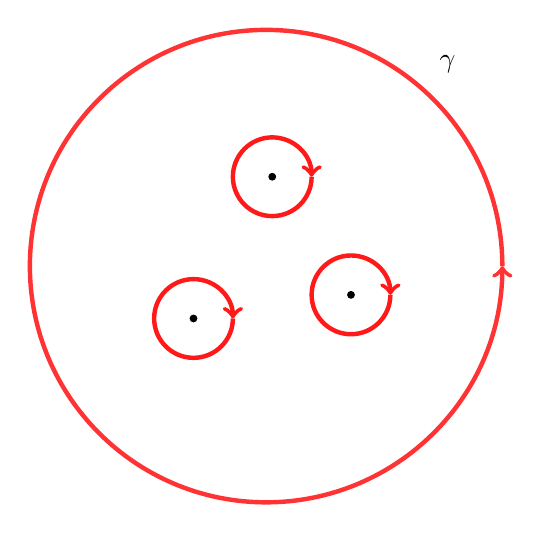
\begin{tikzpicture}
	\coordinate (A) at (0, 0);
	\coordinate (B) at (1,1.8);
	\coordinate (C) at (2, .3);
	\foreach \n in {(A), (B), (C)}
		\draw[color=red!90, ultra thick, ->] \n ++ (0:.5) arc (360:0:.5);
	\foreach \n in {(A), (B), (C)}
		\node at \n [circle,fill,inner sep=1pt]{};
	\draw[color=red!80, ultra thick, ->] (0.922, 0.665)  ++ (0: 3) arc (0:360: 3);
	\node[above right] at (3, 3) {$\LARGE{\gamma}$};
	\end{tikzpicture}

	\medskip
	\small{A visual interpretation of the Cauchy Residue Theorem}
}

\end{document}
